\chapter{Descripción del problema}
\label{descripción}
El modelo implementado se puede resumir como un espacio aéreo dividido en diferentes sectores por el que viajan una serie de aviones. Los vuelos parten y finalizan de un aeropuerto, y tienen una serie de rutas para llegar a su destino.\\
El objetivo del problema es encontrar una solución factible al mayor número de vuelos cumpliendo una serie de restricciones. Las entidades de las que se compone el modelo son las siguientes:

\section{Sectores}
Representan las diferentes zonas en las que dividimos el espacio aéreo. Los sectores tienen un límite de capacidad, de modo que para un instante e tiempo $t$ solo puede haber un número $n$ de vuelos simultáneamente en un sector. De este modo, si un vuelo tiene programado una ruta en un momento de tiempo que pasa por un sector que está al límite de su capacidad, esa ruta no será válida, por lo que tendrá que intentar retrasar su ruta, usar una ruta alternativa, y si no tiene otra opción, cancelarse.\\
Para las pruebas que hemos realizado se ha considerado el escenario más restrictivo posible: la capacidad de un sector en cada instante de tiempo es 1.

\section{Waypoints}
Los waypoints representan los puntos de ruta en las trayectorias de los vuelos a través de los sectores. Dependiendo de su ubicación, los waypoints pueden estar en el interior del sector, por ejemplo en el caso de los aeropuertos, o en la intersección entre dos o más sectores para simular el paso de un sector a otro.


\begin{figure}[H]
	\begin{center}
		\centering
		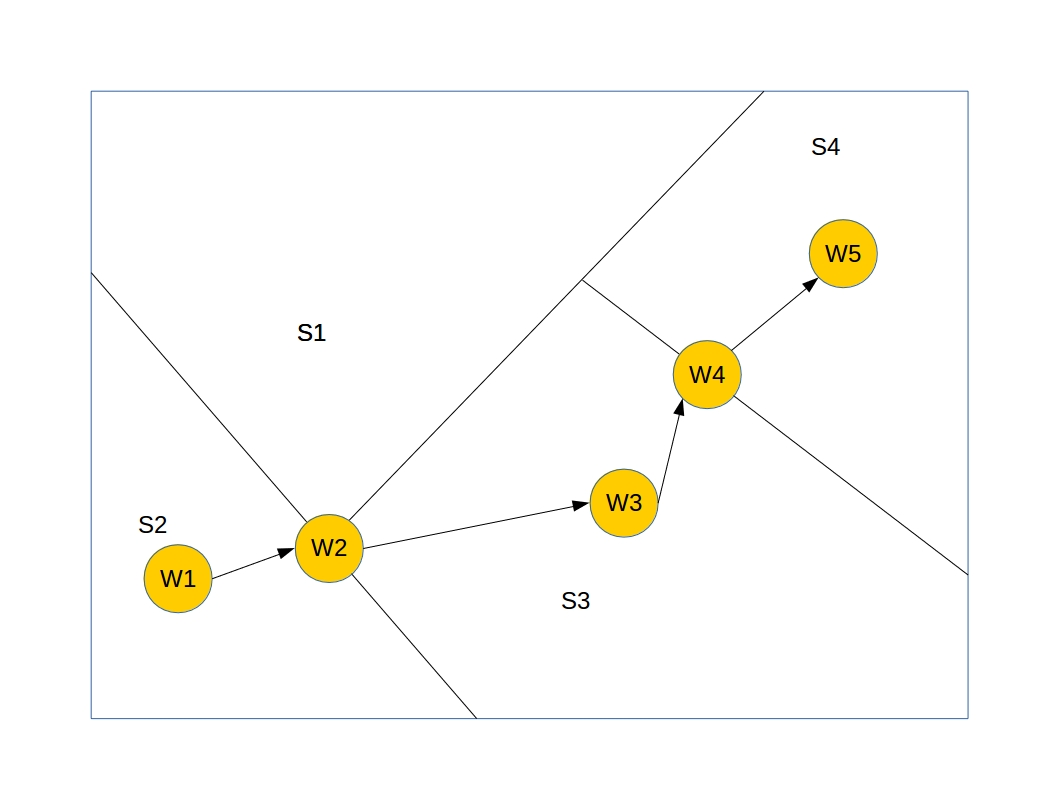
\includegraphics[width=0.9\textwidth]{./imagenes/descripcion_problema/sectoresYWaypoints.jpg}
		\caption{Ejemplo sectores y waypoints}
		\label{fig: Ejemplo sectores y waypoints}
	\end{center}
\end{figure}


\section{Vuelos}
Los vuelos son los elementos que tenemos que maximizar. Tienen una serie de rutas o trayectorias preestablecidas, las cuales siempre empiezan y finalizan en un aeropuerto. Cada vuelo tiene una ruta predefinida, que será siempre igual o mejor (más rápida) que el resto de sus rutas.\\
Además, los vuelos tienen un coste de cancelación y están asociados a determinadas aerolíneas. En este problema consideramos que el todos los vuelos son iguales en importancia, por tanto el coste de cancelación de todos ellos es el mismo, independientemente de la longitud de su ruta, sectores que atraviesa, momento de despegue, etc.\\

Los vuelos a los que sí se les encuentre solución podrán ser  de diferentes tipos:
\begin{itemize}
	\item \textbf{Solución por defecto:} la solución del vuelo es la ruta inicial sin retrasos. Es el mejor resultado posible.
	\item \textbf{Retrasado:} se encuentra una solución factible en la ruta por defecto del vuelo, pero se ha producido un retrasos entre alguno de sus waypoints.
	\item \textbf{Desviado:} la solución encontrada para el vuelo no es la ruta a priori. Puede ser tan corta como la solución por defecto.
\end{itemize}


\section{Rutas}
Las rutas son el conjunto de trayectorias que tiene un vuelo para llegar desde su aeropuerto de origen al de destino. Una de las características más importantes del modelo es que se permite que un vuelo pueda retrasar su trayecto entre 2 waypoints, normalmente para no coincidir en el tiempo y el espacio con otro vuelo o porque el sector al que intenta acceder está sobrecargado. Por tanto en cada trayectoria entre waypoints se permite un retraso máximo, de forma que entre 2 waypoints un vuelo puede recorrer esa distancia entre
\begin{equation}
[T_{mín} , T_{máx}]
\end{equation}

donde 	$T_{mín}$ y $T_{máx}$ son el tiempo mínimo y máximo en el que un vuelo puede ir desde un waypoint a otro, respectivamente.

 En el problema representamos las rutas como un grafo ponderado y dirigido, en el que el coste de cada arista coincide con el intervalo de valores entre los cuales un vuelo puede hacer el trayecto entre 2 waypoints.\\
Para modelar que los aeropuertos no tienen capacidad, creamos unos waypoints $aeropuerto'$ que simulan el waypoint en el que los vuelon aterrizan o despegan (estos waypoints sí que tienen las restricciones habituales del resto de waypoints).

Por ejemplo, un vuelo entre 2 aeropuertos con un waypoint entre ellos en el que se permita en cada trayectoria un retraso de 1, daría como resultado el siguiente grafo:
\begin{figure}[H]
	\centering
	\documentclass{standalone}
\usepackage{tikz}
\begin{document}
\begin{tikzpicture}[->,>=stealth',shorten >=1pt,auto,node distance=3cm,
thick,main node/.style={circle,draw,font=\sffamily\Large\bfseries}]

\node[main node] (1) {$A1$};
\node[main node] (2) [right of=1] {$A1'$};
\node[main node] (3) [right of=2] {$W1$};
\node[main node] (4) [right of=3] {$A3'$};
\node[main node] (5) [right of=4] {$A3$};


\path[every node/.style={font=\sffamily\small}]
(1) edge node {$\{0,1\}$} (2)
(2) edge node {$\{1,2\}$} (3)
(3) edge node {$\{1,2\}$} (4)
(4) edge node {$0$} (5);
\end{tikzpicture}
\end{document}
	\caption{Ejemplo ruta de un vuelo}
	\label{fig: Ejemplo ruta de un vuelo}
\end{figure}

En este ejemplo, el retraso entre $A1$ y $A1'$ representa el retraso en tierra que se permite para el vuelo. El retraso entre los nodos $A3'$ y $A3$, al igual que en cualquier conexión entre los nodos $aeropuerto_aterrizaje'$ y $aeropuerto_aterrizaje$ será siempre 0, ya que no tiene sentido que un vuelo que llega a su aeropuerto de destino retrase su ruta.


\section{Waypoint Route}
Los waypoint route son la entidad que representa los waypoints en diferentes instantes de tiempo. Los waypoint routes son necesarios para crear el grafo de recorridos \textit{completo} de un vuelo, ya que si en alguno de sus trayectos un vuelo permite algún retraso, obtendremos que las aristas del grafo representan a un conjunto de valores.\\

Para crear el grafo que represente las posibles rutas de un vuelo y todos sus posibles retrasos, tenemos que crear un nodo por cada posible waypoint en cada posible instante de tiempo $t$. De esta forma, tendremos un grafo con un conjunto de nodos de la forma $W_{t}$, siendo $W$ el nombre del waypoint y $t$ el instante de tiempo. De esta forma se obtiene que un vuelo puede estar en el mismo waypoint en diferentes momentos de tiempo si se ha elegido otra ruta más larga o se ha producido un retraso.\\

En el ejemplo de \autoref{fig: Ejemplo ruta de un vuelo}, la forma expandida del grafo sería (suponiendo que el vuelo despega en el instante $t=0$): 
\begin{figure}[H]
	\centering
	\documentclass{standalone}
\usepackage{tikz}
%\usetikzlibrary{...}
\begin{document}
	\begin{tikzpicture}[->,>=stealth',shorten >=1pt,auto,node distance=3cm,
	thick,main node/.style={circle,draw,font=\sffamily\Large\bfseries}]
	
	\node[main node] (1) {A1};
	\node[main node] (2) [above right of=1] {$A1'_{0}$};
	\node[main node] (3) [below right of=1] {$A1'_{1}$};
	\node[main node] (4) [above right of=2] {$W1_{2}$};
	\node[main node] (5) [below right of=2] {$W1_{3}$};	
	\node[main node] (6) [above right of=4] {$A3'_{4}$};
	\node[main node] (7) [below right of=4] {$A3'_{5}$};		
	\node[main node] (8) [below right of=5] {$A3'_{6}$};		
	\node[main node] (9) [below right of=3] {$W1_{4}$};		
	\node[main node] (10) [below right of=9] {$A3'_{7}$};		
	\node[main node] (11) [below right of=7] {A3};		
	
	\path[every node/.style={font=\sffamily\small}]
	(1) edge node {0} (2)
	edge node {1} (3)
	(2) edge node {2} (4)	
	edge node {3} (5)
	(3) edge node {2} (5)
	edge node {3} (9)	
	(4) edge node {2} (6)	
	edge node {3} (7)
	(5) edge node {2} (7)
	edge node {2} (8)
	(9) edge node {2} (8)
	edge node {3} (10)
	(6) edge node {0} (11)
	(7) edge node {0} (11)
	(8) edge node {0} (11)
	(10) edge node {0} (11);	
	\end{tikzpicture}
\end{document}




	\caption{Ejemplo grafo de recorridos de un vuelo}
	\label{fig: Ejemplo grafo de recorridos de un vuelo}
\end{figure}

Un vuelo puede además tener más de una ruta. En este caso el grafo de rutas tendrá más de un camino para llegar al nodo de destino:
\begin{figure}[H]
	\centering
	

\documentclass{standalone}
\usepackage{tikz}
%\usetikzlibrary{...}
\begin{document}
		\begin{tikzpicture}[->,>=stealth',shorten >=1pt,auto,node distance=3cm,
		thick,main node/.style={circle,draw,font=\sffamily\Large\bfseries}]
		
		\node[main node] (1) {$A1$};
		\node[main node] (2) [right of=1] {$W1$};
		\node[main node] (3) [right of=2] {$A3$};
		\node[main node] (4) [below of=2] {$W2$};

		
		\path[every node/.style={font=\sffamily\small}]
		(1) edge node {$\{2,3\}$} (2)
		(2) edge node {$\{1,2\}$} (3)
		(1) edge node {$\{3,5\}$} (4)
		(4) edge node {$\{1,2\}$} (3);
		
		\end{tikzpicture}
\end{document}
	\caption{Ejemplo vuelo con 2 rutas}
	\label{fig: Ejemplo vuelo con 2 rutas}
\end{figure}

Su grafo de recorridos se compondría de forma análoga a los anteriores:
\begin{figure}[H]
	\centering
	\documentclass{standalone}
\usepackage{tikz}
%\usetikzlibrary{...}
\begin{document}
	\begin{tikzpicture}[->,>=stealth',shorten >=2pt,auto,node distance=4cm,
	thick,main node/.style={circle,draw,font=\sffamily\Large\bfseries}]
	
	\node[main node] (1) {A1};
	\node[main node] (2) [above right of=1] {$A1'_{0}$};
	\node[main node] (3) [below right of=1] {$A1'_{1}$};
	\node[main node] (4) [above right of=2] {$W1_{2}$};
	\node[main node] (5) [below right of=2] {$W1_{3}$};	
	\node[main node] (6) [above of=7] {$A3'_{4}$};
	\node[main node] (7) [above left of=11] {$A3'_{5}$};		
	\node[main node] (8) [below left of=11] {$A3'_{6}$};		
	\node[main node] (9) [below left of=10] {$W1_{4}$};		
	\node[main node] (10) [below of=8] {$A3'_{7}$};		
	\node[main node] (11) [below right of=7] {A3};		
	\node[main node] (12) [above left of=6] {$W2_{3}$};		
	\node[main node] (13) [below left of=8] {$W2_{4}$};	

	\path[every node/.style={font=\sffamily\small}]
	(1) edge node {0} (2)
	edge node {1} (3)
	(2) edge [blue] node {2} (4)	
	edge [blue] node {3} (5)
	edge [red] node {3} (12)
	edge [red] node {4} (13)
	(3) edge [blue] node {2} (5)
	edge [blue] node {3} (9)	
	edge [red] node {3} (13)

	(4) edge [blue] node {2} (6)	
	edge [blue] node {3} (7)
	(5) edge [blue] node {2} (7)
	edge [blue] node {2} (8)
	(9) edge [blue] node {2} (8)
	edge [blue] node {3} (10)
	(6) edge node {0} (11)
	(7) edge node {0} (11)
	(8) edge node {0} (11)
	(10) edge node {0} (11)
	(12) edge [red] node {1} (6)
	(13) edge [red] node {1} (7)
		;	
	\end{tikzpicture}
\end{document}




	\caption{Ejemplo grafo recorridos con 2 rutas: ruta 1 en \textcolor{blue}{azul} y ruta 2 en \textcolor{red}{rojo}  }
	\label{fig: Ejemplo grafo recorridos con 2 rutas}
\end{figure}
\section{Descripción del modelo}
Por tanto, el modelo se puede expresar como
\begin{itemize}
	\item \textbf{Función objetivo: }hay que maximizar el número de vuelos a los que se les encuentra una solución factible.\\
	 Dado que los vuelos no tienen solución binaria (cancelado/con solución), sino que dentro de las soluciones factibles hay unas mejores que otras, se ha creado un sistema de evaluación de vuelos con solución factible: los vuelos colocados en su solución a priori aportan 5 pts, los retrasados 3, los desviados en tiempo 2 y los desviados y retrasados 1.\\
	 Este sencillo sistema se ideó para evaluar lo factible que es una solución, ya que como se explicó anteriormente no estamos utilizando el coste de cancelación (en ese caso se trataría de un problema de minimización de costes, en vez de maximizar la solución).
	\item \textbf{Restricciones:} el modelo tiene tan sólo dos:
	\begin{enumerate}
		\item Para cualquier instante de tiempo $t$, no puede haber más de 1 vuelo en un arco que conecta 2 waypoints. 
		\item Dado cualquier instante de tiempo $t$, no puede haber más de $n$ vuelos simultáneamente en el mismo sector. Aunque $n$ es un parámetro variable, todas las pruebas que hemos realizado hemos usado $n=1$, poniéndonos así en el caso más estricto de todos.
	\end{enumerate}
	
	
\end{itemize}

\section{Estructura de clases}
El esquema de clases que se ha creado para modelar las entidades del modelo corresponden con los siguientes (para más información consultar en el \autoref{anexo2}):
\textcolor{red}{IMAGEN CON DIAGRAMA DE CLASES}